
\documentclass{article}
\usepackage[letterpaper,top=0.5in,bottom=0.5in,left=.5in,right=.5in,includeheadfoot]{geometry}
\usepackage{amssymb,amsmath}
\usepackage{parskip}
\usepackage{fancyhdr}
\usepackage{tabu}
\usepackage{enumerate}
\usepackage{graphicx}
\usepackage{tikz}
\usepackage{multicol}
\usepackage{color}
\usepackage{soul}
\usepackage{changepage}
\usepackage{endnotes}
% \usepackage{dblfnote}
\usepackage{hyperref}
\hypersetup{colorlinks=true,urlcolor=blue}

\renewcommand{\baselinestretch}{1.3}
\pagestyle{fancy}
\fancyfoot{}
\renewcommand{\headrulewidth}{0pt}
\setlength{\headheight}{0pt}

\fancypagestyle{firstpage}{
  \fancyhead{}
  \fancyfoot{}
}

\usepackage{titlesec}

\titlespacing\title{0pt}{0pt plus 4pt minus 2pt}{-5pt plus 2pt minus 2pt}
\titlespacing\section{0pt}{-8pt plus 4pt minus 2pt}{-6pt plus 2pt minus 2pt}
\titlespacing\subsection{0pt}{0pt plus 4pt minus 2pt}{-6pt plus 2pt minus 2pt}
\titlespacing\subsubsection{0pt}{0pt plus 4pt minus 2pt}{-5pt plus 2pt minus 2pt}


\newcommand{\TODO}{\textcolor{red}{\textbf{\hl{TODO}}}}

\begin{document}
% \thispagestyle{firstpage}
% \PrintFirstHeader{}
% \pagebreak


%================================ COVER PAGE ================================

%*********** Use this for project proposal (comment out in project report) ************
\emph{\footnotesize{CIS 520 Spring 2019, Project Report}}

%*********** Use this for project report (comment out in project proposal) ************
%\emph{\footnotesize{CIS 520 Spring 2018, Project Report}}

\vspace{12pt}

%Fill in your project title
\textbf{\Large{Project Title}}

\vspace{1cm}

\textbf{Team Members:} \\
%Fill in your team details; remove any lines that are not needed
Monal Garg (PennKey: \texttt{mgarg}; Email: \texttt{mgarg@sas.upenn.edu}) \\
Amit Gupta (PennKey: \texttt{akgupta}; Email: \texttt{akgupta@seas.upenn.edu}) \\
Aashish Jain (PennKey: \texttt{aashj99}; Email: \texttt{aashj99@seas.upenn.edu}) \\
Moksh Jawa (PennKey: \texttt{moksh}; Email: \texttt{moksh@seas.upenn.edu})

%---

\vspace{2cm}

%*********** Comment out the following for the proposal; uncomment and fill in all details for the project report ***********

\textbf{Assigned Project Mentor:}

%Fill in assigned TA name
Jane Lee

\vspace{1cm}

\textbf{Team Member Contributions:}

%Fill in team member contributions
\begin{center}
\begin{tabular}{|l|l|}
\hline
Team Member & Contributions \\
\hline
Monal Garg & Past Work, Solution Approach, Machine Learning Algorithms, Visualizations, Report \\
  & (continue if needed) \\
\hline
Amit Gupta & Problem Formulation, Algorithms Plan for Use, Machine Learning Algorithms, Visualizations, Report \\
  & (continue if needed) \\
\hline
Aashish Jain & Data Cleaning, Data Stitching, Machine Learning Algorithms, Visualizations, Report \\
  & (continue if needed) \\
\hline
Moksh Jawa & Data Cleaning, Data Stitching, Machine Learning Algorithms, Visualizations, Report \\
  & (continue if needed) \\
\hline
\end{tabular}
\end{center}

\vspace{12pt}

\textbf{Code Submission:}

\normalsize{Public GitHub Repo can be found at\href{https://github.com/akgpta/CIS520-Final-Project}{https://github.com/akgpta/CIS520-Final-Project}}



\newpage
\tableofcontents
\newpage

\section{Abstract}
Suicide is a major public health concern worldwide and varies from country to country. Because living in a different country and environment can greatly impact one's lifestyle, we were interested in collecting national data that could impact one's life over several years to better understand suicide rates internationally. With this data, we were interested in finding what factors could be possiblely linked to certain suicide rate trends. To do this, we ran $k$-nearest neighbors, linear regression, and neural networks on the data... \TODO

\begin{multicols}{2}
\section{Introduction}
\subsection{Problem Motivation} Unfortunately, it is a sad reality that many individuals each year commit suicide. We in the U.S. are slowly being aware of this issue, but we wanted to understand suicide rates internationally. Especially, we wanted to look at these rates as they related to common features of each country, such as GDP, unemployment, and alcohol consumption. At a high-level we wanted to draw out any meaningful relationship between these macro features and suicide rates.
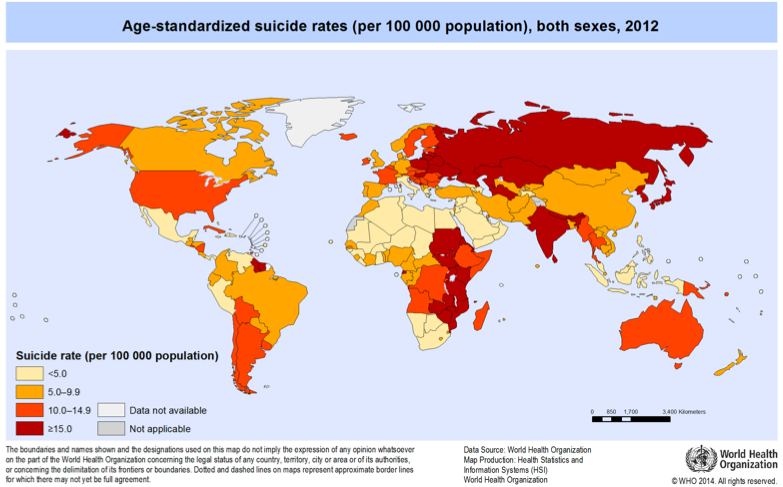
\includegraphics[width=\columnwidth]{2012-data-vis-map.png}
\subsection{Data Set and Source} Our project grew from an intriguing 
World Health Organization data set will well over 35 years of suicide rates by country broken up by demographics.  \endnote{https://www.kaggle.com/szamil/who-suicide-statistics}. In an effort to extend existing analyses though, we actually sources global data from a variety of sources. This included a FiveThirtyEight data set on alcohol consumptixon \endnote{https://www.kaggle.com/fivethirtyeight/fivethirtyeight-alcohol-consumption-dataset}. We also incorporated a World Bank Data Set on Youth Unemployment \endnote{https://www.kaggle.com/sovannt/world-bank-youth-unemployment} and another from the World Bank on population, fertility, and life expectancy \endnote{https://www.kaggle.com/gemartin/world-bank-data-1960-to-2016}. A lot of the work done was with respect to time series and things like that. What we wanted to do, though, was take a look at combining data from multiple sources. 
Our project team sought to understand a little bit more about the intricacies of sourcing data from multiple places. This proved to be a difficult challenge.  
\subsection{Summary Statistics} 
We've provided summary statistics for 4 of the datasets we will be using in our project shown in Tables \hyperref[summary-statistic-table-alcohol]{0}, \ref{summary-statistic-table-youth-unemployment}, \ref{summary-statistic-table-fertility}, \ref{summary-statistic-table-life}, some of which are located in the appendix.

\begin{adjustwidth}{8px}{}
\begin{tabular}{|l|l|}
\hline
Statistic          & Average liters/person/year \\ \hline
Min                & 0                          \\ \hline
Max                & 14.4                       \\ \hline
Mean               & 4.71                       \\ \hline
Median             & 4.2                        \\ \hline
Standard Deviation & 3.77                       \\ \hline
\multicolumn{2}{c}{Table 0: Alcohol Consumption by Country} 
\label{summary-statistic-table-alcohol}
\end{tabular}
\end{adjustwidth}


\section{Related Work}
\subsection{Related to Models} 

Among the papers that analzyed economic factors, a regression model seemed to be the popular choice of method. For example, Pandey and Kaur paper used a Auto-Regressive Distributed Lag (ARDL) model \endnote{https://crawford.anu.edu.au/acde/asarc/pdf/papers/2009/WP2009/{\_}08.pdf}. 

Most of the articles concerning the relationship of suicide rate and alcohol consumption related trends from a biological perspective utilized relatively simple statistical analysis \endnote{https://www.ncbi.nlm.nih.gov/pubmed/9229027}. Whereas medical research that involved more complex forms of data such as fMRI brain scans utilized algorithms such as Gaussian Naive Bayes \endnote{https://nocklab.fas.harvard.edu/files/nocklab/files/just{\_}2017{\_}machlearn{\_}suicide{\_}emotion{\_}youth.pdf}.

\subsection{Related to Problem} 

During our research, we came across multiple research papers that analyze the correlation between suicide rates and either economical, behavioral, medical, or psychological factors. For example, the Pandey and Kaur paper investigates suicidal trend and economic determinants in an Indian population\endnote{https://crawford.anu.edu.au/acde/asarc/pdf/papers/2009/WP2009/{\_}08.pdf}. Whereas articles published in medical journals explored suicide with alochol/drug consumption, psychotic behavior, brain scans, etc \endnote{https://www.ncbi.nlm.nih.gov/pmc/articles/PMC2872355/}. 

However, most papers tend to focus on either the economic or behavioral/medical factors. As suicide is likely governed by multiple factors, we seek to investigate this problem through a more holistic approach by simultaneously analyzing both medical, behavioral, and economic factors. Through this application of machine learning, we hope to gain insight on the relative role each factor plays in suicide and about the interaction of these factors. 

Moreover, most papers perform a time series analysis. We provide a different approach by analyzing the data by country. Papers that do focus on certain regions usually provide analyses on one country or a specific region, whereas we will analyze global statistics. 


\section{Problem Formulation and Data} 
\subsection{Data Processing Needed} Our data came in a variety of comma-separated formats. A lot of countries were labelled in differing manner and years were often a column and other times a point in a row. We used Excel Pivot Tables to make these more easily parsable and standardized. Later, blanks and other issues with inconsistencies are removed with Python to get an aggregated set of data. Other pre-processing includes removing blanks, reconciling some country names such as (Trinidad \& Tobago vs. Trinidad and Tobago).
\TODO : talk about cleaning (Pandas, Excel)
\subsection{Inputs, Outputs} Inputs are a variety of real-valued data points tied to the country. They are described above, but it remains to see which we might have to throw out due to excessive blanks. Most are also measured for a specific year, however some are just duplicated across all years (e.g. Alcohol Consumption). Outputs are a model, which given a countries characteristic features, can predict suicide rates. We have suicide rates by gender (as well as age demographics), so we may also seek a model which predicts a rate for male suicides and a rate for female suicides.
\subsection{Performance Measures} \TODO update to be what we acutally used
Given the regression nature of this problem, we believe a squared loss model is appropriate. 
\TODO: address her comments

\section{Solution Methods and Algorithms}
\TODO : update to what we actually did - why we choose, how they were implemented, what languages 
\TODO : THIS WHOLE SECTION NEEDS TO BE REWRITTEN FOR WHAT WE ACTUALLY DID \TODO
\subsection{Algorithms Used} \TODO describe algorithms, implementations, etc.. \TODO We will start with least squares regression in unregularized, $L_1$ regularized, and $L_2$ regularized forms. We are not certain whether any of our features will be overly correlated so the unregularized least squares regression may fail. We also seek to explore Nearest Neighbor methods, but not with vanilla Euclidean distance, but with feature weighted scaling on the distances. Lastly, we will consider using decision stubs as features and feeding the transformed input space into another learning model, perhaps Neural Nets.

\section{Experimental Design and Results}
\subsection{Experiments}
\TODO Describe how you set up your experiments, including choice
of training/testing data, choice of parameters, etc, in a way that your results can be reproduced \TODO
\subsection{Results}
\TODO training/testing times, possible visualizations of results including both examples of good
performance and examples of what types of errors are made, etc. \TODO


\includegraphics[width=\columnwidth]{geo-bee.jpg}
The best predictor of suicide rates is the country label itself. Suicide rates in Ghana in 2013 are going to look like suicide rates in Ghana in 2012 most. Modelling this regression outcome as independent draws disregards the time series data and correlation of examples. As such, nearest neighbors performs exceptionally well, since it just recognized the country through these 8 input features. 


\section{Discussion and Reflections}
\TODO : Discussion about any sort of data specific things we gleaned, I already did the meta analysis \TODO
\subsection{Takeaways}
This project was certainly an adventure in machine learning. Let us recall some of the lines from what we set out to do. Note, these were established a priori in our proposal: \textit{``at a high-level we wanted to draw out any meaningful relationship between these macro features and suicide rates'}' and \textit{``we hope to gain insight on the
relative role each factor plays in suicide and about the interaction of these factors''}. We were thinking that a model would illimuniate which features wre coupled with suicide rates. As the project continued though, as noted in our Results section, models were essentially using the features to identify individual countries. We are careful in this report to not conflate correlation with causation and, as such, have left out implications of this country-recognizer model built. \\
Reflecting on our goal, it seems the problem we have chosen to tackle doesn't really make sense from a machine learning perspective. Sure, the factors we have chosen can be used to generate a model which fairly reliably outputs suicide rates. However, this correlation should not be taken to imply causation or even anything close to that. From a model story perspective, suicide rates are affected by many factors exogenous to our world of data. \\
When you consider some sort of underlying sampling distribution assumptions on the data, it doesn't make sense that suicide rates for countries on different continents with different socioeconomic statuses are coming from one distribution. Although this seems to say that this project wasn't an effective learning opportunity, we as a team feel quite the opposite. \\
There are a finite number of countries in the world. In fact, there are 195 countries in the world. As such, worries about reasonable time computation, tractability, and other aspects of problems centered on larger data (think users of Netflix or game states) does not really factor in here. Had we as a group had more experience at the start of this project, perhaps we would have foreseen the uniqueness of countries leading to a model which could basically be a geography bee champion. However, we feel that the machine learning exercises carried out during the course of this project deepened our understanding of course algorithms, implications, and relevant considerations.




% \subsection{Pre-Milestone Meeting Goals} 

% Our goal before our milestone meeting is have the data completed clean and visualized. Additionally, we plan to have k-Nearest Neighbors and Least Squares Regression implemented, visualized, and results recorded. Note that our k-Nearest Neighbor implementation will have weighted scaling based on features rather than Euclidean distance.

% \subsection{Timelines}

% After our milestone meeting, we will have exactly 3 weeks. The first week will involve implementing our last approach of decision stubs as features and feeding them into neural nets. The second week will involve finetuning and evaluating our models. The last week will be for writing up the report

\section{Acknowledgements} \TODO N/A

\end{multicols}

\pagebreak

\section{References} \TODO: update? \theendnotes

\section{Appendix} 
\begin{table}[ht]
\centering
\begin{tabular}{|l|l|l|l|l|l|}
\hline
          &  \multicolumn{5}{c|}{Youth Unemployed} \\ \hline
Statistic          &  \%  2010 &  \% 2011 &  \% 2012 &  \%  2013 & \% 2014 \\ \hline
Min                & 0.6999                    & 0.6999                    & 0.5                       & 0.6999                    & 0.6999                    \\ \hline
Max                & 57.2                      & 57.1                      & 61.7                      & 58                        & 57.9                      \\ \hline
Mean               & 17.89                     & 17.9                      & 18.15                     & 18.1                      & 17.94                     \\ \hline
Median             & 14.9                      & 14.52                     & 14.4                      & 14.1                      & 14.12                     \\ \hline
Standard Deviation & 10.54                     & 10.88                     & 11.43                     & 11.67                     & 11.55                     \\ \hline
\end{tabular}
\caption{Youth Unemployment by Country}
\label{summary-statistic-table-youth-unemployment}
\end{table}
\begin{table}[ht]
\centering
\begin{tabular}{|l|l|l|l|l|l|}
\hline
          &  \multicolumn{5}{c|}{Fertility Rates} \\ \hline
Statistic          &  \%  2010 &  \% 2011 &  \% 2012 &  \%  2013 & \% 2014 \\ \hline
Min                & 1.06                   & 1.11                   & 1.16                   & 1.13                   & 1.21                   \\ \hline
Max                & 7.49                   & 7.46                   & 7.42                   & 7.38                   & 7.34                   \\ \hline
Mean               & 2.91                   & 2.88                   & 2.84                   & 2.81                   & 2.79                   \\ \hline
Median             & 2.41                   & 2.37                   & 2.34                   & 2.34                   & 2.33                   \\ \hline
Standard Deviation & 1.45                   & 1.42                   & 1.39                   & 1.37                   & 1.34                   \\ \hline
\end{tabular}
\caption{Fertility Rates by Country}
\label{summary-statistic-table-fertility}
\end{table}
\begin{multicols}{2}


\end{multicols}
\begin{table}[ht]
\centering
\begin{tabular}{|l|l|l|l|l|l|}
\hline
          &  \multicolumn{5}{c|}{Life Expectancy} \\ \hline
Statistic          &  \%  2010 &  \% 2011 &  \% 2012 &  \%  2013 & \% 2014 \\ \hline
Min                & 47.56                  & 48.284                 & 49.041                 & 49.825                 & 50.621                 \\ \hline
Max                & 82.9780488             & 83.4219512             & 85.4170732             & 83.8317073             & 83.9804878             \\ \hline
Median             & 72.2783848             & 72.4719847             & 72.657                 & 72.786                 & 72.9707317             \\ \hline
Standard Deviation & 8.34929356             & 8.19102272             & 8.04819537             & 7.89104622             & 7.80484223             \\ \hline
\end{tabular}
\caption{Life Expectancy by Country}
\label{summary-statistic-table-life}
\end{table}





\end{document}
